% chap09 - Systems of ODEs
% Last edited:

\chapter{Systems of ODEs}

\section{Matrices}

A matrix is a two-dimensional version of a vector. Like a vector,
it contains elements that are identified by indices. The difference
is that the elements are arranged in rows and columns, so it takes
{\em two} indices to identify an element.

One of many ways to create a matrix is the {\tt magic} function,
which returns a ``magic'' matrix with the given size:

\begin{verbatim}
octave:1> M = magic(3)

M = 8   1   6
   3   5   7
   4   9   2
\end{verbatim}

If you don't know the size of a matrix, you can use {\tt whos} to
display it:

\begin{verbatim}
octave:1> whos
 Name    Size          Bytes Class
 M      3x3            72 double array
\end{verbatim}

Or the {\tt size} function, which returns a vector:

\begin{verbatim}
octave:1> V = size(M)

V = 3   3
\end{verbatim}

The first element is the number of rows, the second is the number of
columns.

To read an element of a matrix, you specify the row and column numbers:

\begin{verbatim}
octave:1> M(1,2)

ans = 1

octave:1> M(2,1)

ans = 3
\end{verbatim}

When you are working with matrices, it takes some effort to remember
which index comes first, row or column. I find it useful to repeat
``row, column'' to myself, like a mantra. You might also find it
helpful to remember ``down, across,'' or the abbreviation RC.

Another way to create a matrix is to enclose the elements in
brackets, with semi-colons between rows:

\begin{verbatim}
octave:1> D = [1,2,3 ; 4,5,6]

D = 1   2   3
   4   5   6

octave:1> size(D)

ans = 2   3
\end{verbatim}


\section{Row and column vectors}

Although it is useful to think in terms of scalars, vectors and matrices,
from Octave's point of view, everything is a matrix. A scalar
is just a matrix that happens to have one row and one column:

\begin{verbatim}
octave:1> x = 5;
octave:1> size(x)

ans = 1   1
\end{verbatim}

And a vector is a matrix with only one row:

\begin{verbatim}
octave:1> R = 1:5;
octave:1> size(R)

ans = 1   5
\end{verbatim}

Well, some vectors, anyway. Actually, there are two kind
of vectors. The ones we have seen so far are called {\bf row vectors},
because the elements are arranged in a row; the other kind are
{\bf column vectors}, where the elements are in a single column.

One way to create a column vector is to create a matrix with only
one element per row:

\begin{verbatim}
octave:1> C = [1;2;3]

C =

   1
   2
   3

octave:1> size(C)

ans = 3   1
\end{verbatim}

The difference between row and column vectors is important in
linear algebra, but for
most basic vector operations, it doesn't matter. When you
index the elements of a vector, you don't have to know what kind
it is:

\begin{verbatim}
octave:1> R(2)

ans = 2

octave:1> C(2)

ans = 2
\end{verbatim}



\section{The transpose operator}

The transpose operator, which looks remarkably like an apostrophe,
computes the {\bf transpose} of a matrix, which is a new matrix
that has all of the elements of the original, but with each row
transformed into a column (or you can think of it the other way around).

In this example:

\begin{verbatim}
octave:1> D = [1,2,3 ; 4,5,6]

D = 1   2   3
   4   5   6
\end{verbatim}

{\tt D} has two rows, so its transpose has two columns:

\begin{verbatim}
octave:1> Dt = D'

Dt = 1   4
   2   5
   3   6
\end{verbatim}

\begin{ex}
What effect does the transpose operator
have on row vectors, column vectors, and scalars?
\end{ex}


\section{Lotka-Voltera}
\label{lotka}

The Lotka-Voltera model describes the interactions between two
species in an ecosystem, a predator and its prey. A common example
is rabbits and foxes.

The model is governed by the following system of differential
equations:

\begin{eqnarray*}
R_t = a R - b R F \\
F_t = e b R F - c F
\end{eqnarray*}
%
where
%
\begin{itemize}
%
\item $R$ is the population of rabbits,
\item $F$ is the population of foxes,
\item $a$ is the natural growth rate of rabbits in the absence of predation,
\item $c$ is the natural death rate of foxes in the absence of prey,
\item $b$ is the death rate of rabbits per interaction with a fox,
\item $e$ is the efficiency of turning eaten rabbits into foxes.
%
\end{itemize}

At first glance you might think you could solve these equations by
calling {\tt ode45} once to solve for $R$ as a function of time and
once to solve for $F$. The problem is that each equation involves
both variables, which is what makes this a {\bf system of equations}
and not just a list of unrelated equations. To solve a system, you
have to solve the equations simultaneously.

Fortunately, {\tt ode45} can handle systems of equations. The
difference is that the initial condition is a vector that contains
initial values $R(0)$ and $F(0)$, and the output is a matrix
that contains one column for $R$ and one for $F$.

And here's what the rate function looks like
with the parameters $a = 0.1$, $b = 0.01$, $c = 0.1$ and $e = 0.2$:

\begin{verbatim}
function res = lotka(t, V)
  % unpack the elements of V
  r = V(1);
  f = V(2);

  % set the parameters
  a = 0.1;
  b = 0.01;
  c = 0.1;
  e = 0.2;
  
  % compute the derivatives
  drdt = a*r - b*r*f;
  dfdt = e*b*r*f - c*f;
  
  % pack the derivatives into a vector
  res = [drdt; dfdt];
end
\end{verbatim}

As usual, the first input variable is time.
The second input variable is a vector with two elements,
$R(t)$ and $F(t)$. I gave it a capital letter to remind me that it
is a vector. The body of the function includes four {\bf paragraphs},
each explained by a comment.

The first paragraph {\bf unpacks} the vector by copying the elements
into scalar variables. This isn't necessary, but giving names to
these values helps me remember what's what. It also makes the third
paragraph, where we compute the derivatives, resemble the mathematical
equations we were given, which helps prevent errors.

The second paragraph sets the parameters that describe the
reproductive rates of rabbits and foxes, and the characteristics of
their interactions. If we were studying a real system, these values
would come from observations of real animals, but for this example
I chose values that yield interesting results.

The last paragraph {\bf packs} the computed derivatives back into a
vector. When {\tt ode45} calls this function, it provides a vector
as input and expects to get a vector as output.

Sharp-eyed readers will notice something different about this line:

\begin{verbatim}
  res = [drdt; dfdt];
\end{verbatim}

The semi-colon between the elements of the vector is not an error. It
is necessary in this case because {\tt ode45} requires the result of
this function to be a column vector.

Now we can run {\tt ode45} like this:

\begin{verbatim}
ode45(@lotka, [0, 365], [100, 10])
\end{verbatim}

As always, the first argument is a function handle, the second is the
time interval, and the third is the initial condition. The initial
condition is a vector: the first element is the number of rabbits at
$t=0$, the second element is the number of foxes.

The order of these elements (rabbits and foxes) is up to you, but
you have to be consistent. That is, the initial conditions you
provide when you call {\tt ode45} have to be the same as the order,
inside {\tt lotka}, where you unpack the input vector and repack
the output vector. Octave doesn't know what these values mean;
it is up to you as the programmer to keep track.

But if you get the order right, you should see something like this:

\beforefig \centerline{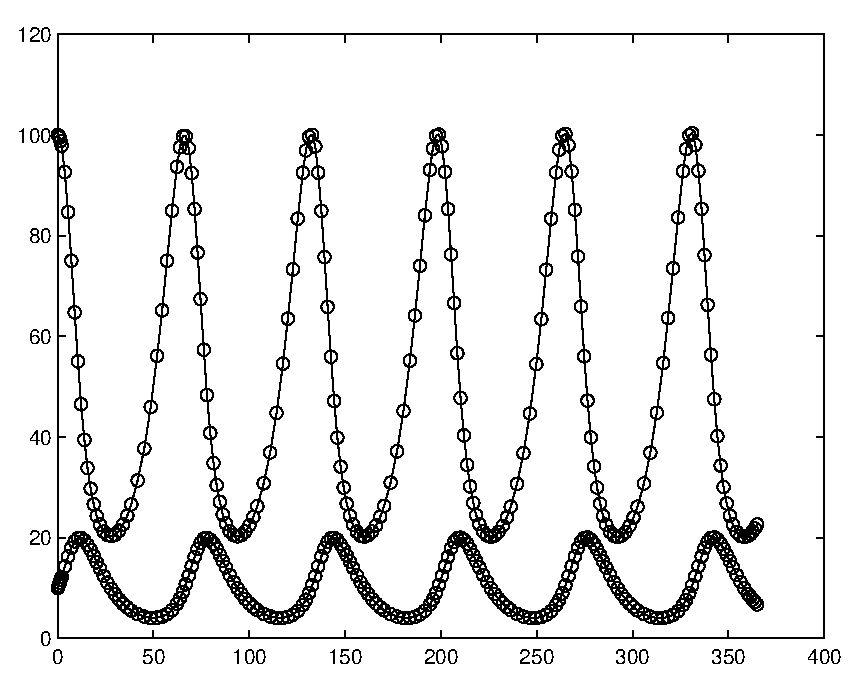
\includegraphics[height=2in]{figs/lotka.eps}}

The x-axis is time in days; the y-axis is population. The top
curve shows the population of rabbits; the bottom curve shows
foxes. This result is one of several patterns
this system can fall into, depending on the starting conditions
and the parameters. As an exercise, try experimenting with
different values.


\section{What can go wrong?}

The output vector from the rate function
has to be a column vector; otherwise you get

\begin{verbatim}
??? Error using ==> funfun/private/odearguments
LOTKA must return a column vector.

Error in ==> ode45 at 173
[neq, tspan, ntspan, next, t0, tfinal, tdir, y0, f0, odeArgs,
odeFcn, ...
\end{verbatim}

Which is pretty good as error messages go. It's not clear {\em why}
it needs to be a column vector, but that's not our problem.

Another possible error is reversing the order of the elements in the
initial conditions, or the vectors inside {\tt lotka}. Again, Octave
doesn't know what the elements are supposed to mean, so it can't catch
errors like this; it will just produce incorrect results.


\section{Output matrices}

As we saw before, if you call {\tt ode45} without assigning the
results to variables, it plots the results. 
If you assign
the results to variables, it suppresses the figure.
Here's what that looks like:

\begin{verbatim}
octave:1> [T, M] = ode45(@lotka, [0, 365], [100, 10]);
\end{verbatim}

You can think of the left side of this assignment as a vector
of variables.

As in previous examples, {\tt T} is a vector of time values where {\tt
ode45} made estimates. But unlike previous examples, the
second output variable is a matrix containing one column for each
variable (in this case, $R$ and $F$) and one row for each time value.

\begin{verbatim}
octave:1> size(M)

ans = 185   2
\end{verbatim}

This structure---one column per variable---is a common way to
use matrices. {\tt plot} understands this structure, so if you
do this:

\begin{verbatim}
octave:1> plot(T, M)
\end{verbatim}

Octave understands that it should plot each column from {\tt M}
versus {\tt T}.

You can copy the columns of {\tt M} into other variables like
this:

\begin{verbatim}
octave:1> R = M(:, 1);
octave:1> F = M(:, 2);
\end{verbatim}

In this context, the colon represents the range from 1 to {\tt end},
so {\tt M(:, 1)} means ``all the rows, column 1'' and
{\tt M(:, 2)} means ``all the rows, column 2.''

\begin{verbatim}
octave:1> size(R)

ans = 185   1

octave:1> size(F)

ans = 185   1
\end{verbatim}

So {\tt R} and {\tt F} are column vectors. 


If you plot these
vectors against each other, like this

\begin{verbatim}
octave:1> plot(R, F)
\end{verbatim}

You get a {\bf phase plot} that looks like this:

\beforefig \centerline{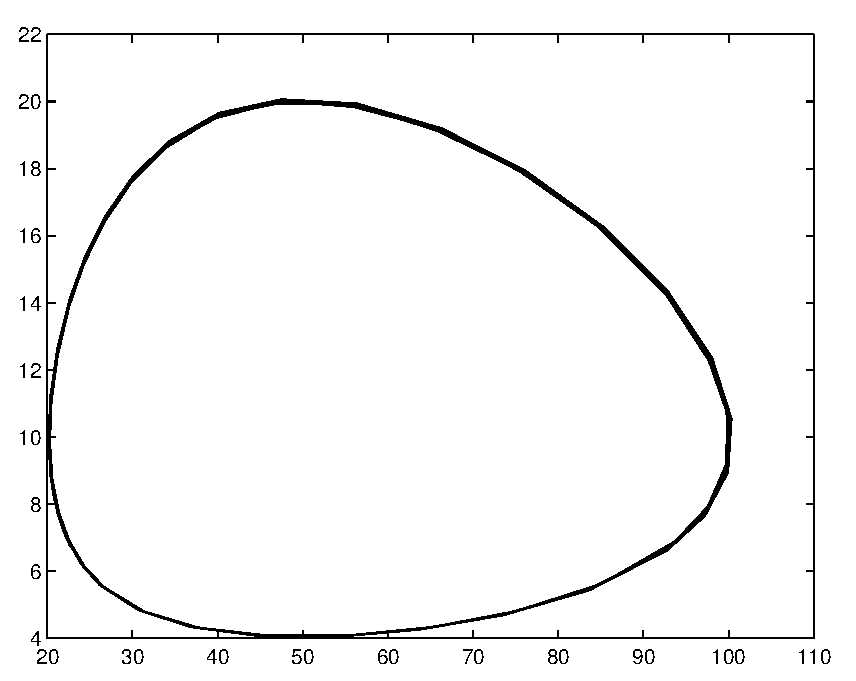
\includegraphics[height=2in]{figs/phase.eps}}

Each point on this plot represents a certain number of rabbits (on the
x axis) and a certain number of foxes (on the y axis).

Since these are the only two variables in the system, each point in
this plane describes the complete {\bf state} of the system.

Over time, the state moves around the plane; this figure shows
the path traced by the state during the time interval. This path
is called a {\bf trajectory}.

Since the behavior of this system is periodic, the resulting
trajectory is a loop.

If there are 3 variables in the system, we need 3 dimensions to show
the state of the system, so the trajectory is a 3-D curve.
You can use {\tt plot3} to trace trajectories in 3 dimensions,
but for 4 or more variables, you are on your own.


\section{Glossary}

\begin{description}

\item[row vector:] In Octave, a matrix that has only one row. 

\item[column vector:] A matrix that has only one column. 

\item[transpose:] An operation that transforms the rows of a matrix
into columns (or the other way around, if you prefer). 

\item[system of equations:] A set of equations written in terms of
a set of variables such that the equations are intertangled.

\item[paragraph:] A chunk of code that makes up part of a function,
usually with an explanatory comment. 

\item[unpack:] To copy the elements of a vector into a set of variables.

\item[pack:] To copy values from a set of variables into a vector. 

\item[state:] If a system can be described by a set of variables,
the values of those variables are called the state of the system.

\item[phase plot:] A plot that shows the state of a system as point
in the space of possible states. 

\item[trajectory:] A path in a phase plot that shows how the state of
a system changes over time.


\end{description}

\section{Exercises}

\begin{ex}

Based on the examples we have seen so far, you would think that
all ODEs describe population as
a function of time, but that's not true.

According to the
Wikipedia\footnote{\url{http://en.wikipedia.org/wiki/Lorenz_attractor}},
``The Lorenz attractor, introduced by Edward Lorenz in 1963, is a
non-linear three-dimensional deterministic dynamical system derived
from the simplified equations of convection rolls arising in the
dynamical equations of the atmosphere. For a certain set of parameters
the system exhibits chaotic behavior and displays what is today called
a strange attractor...''

The system is described by this system of differential equations:
%
\begin{eqnarray}
x_t &=& \sigma (y - x) \\
y_t &=& x (r - z) - y  \\
z_t &=& xy - b z
\end{eqnarray}
%
Common values for the parameters are $\sigma = 10$, $b = 8/3$ and $r=28$.

Use {\tt ode45} to estimate a solution to this
system of equations. 


\begin{enumerate}

\item The first step is to write a function named {\tt lorenz} that
takes {\tt t} and {\tt V} as input variables, where the components
of {\tt V} are understood to be the current values of {\tt x},
{\tt y} and {\tt z}. It should compute the corresponding derivatives
and return them in a single column vector.

\item The next step is to test your function by calling it from
the command line with values like
$t=0$, $x=1$, $y=2$ and $z=3$? Once you get your function working,
you should make it a silent function before calling {\tt ode45}.

\item Assuming that Step 2 works, you can use {\tt ode45}
to estimate the solution for the time interval $t_0 = 0$, $t_e = 30$
with the initial condition $x=1$, $y=2$ and $z=3$.

\item Use {\tt plot3} to plot the trajectory of
$x$, $y$ and $z$.

\end{enumerate}

\end{ex}
